\chapter{Requirements}

	\section{Features}
	
	The following feature list is the one proposed for the \ac{AWESOME} prototype.
	The project follows this feature set as a baseline set of requirements.
	
	\begin{itemize}
		\item \textbf{Automatic questionnaire generation per-student} - Generate unique questionnaires per-student, depending on their modules and lecturers.
		\item \textbf{The ability to generate quick mid-term questionnaires} - A one question per module survey with a one to five scale from `This module is going well' to `This module has problems'.
		\item \textbf{No need to type in registration details} - Import of module registration data via \ac{ASTRA} \ac{CSV} export.
		\item \textbf{Targeted follow-up reminder emails} - Only send reminder emails to respondents who have yet to complete their questionnaire.
		\item \textbf{Anonymous responses} - Ability to know which particular student has, or has not completed the questionnaire, but not who has said what.
		\item \textbf{Visually appealing analytics} - Reports available to staff on a by-module, by-department, and by-scheme basis, with graphs and textual responses laid out nicely.
	\end{itemize}

	\section{Development Practices}
	
	\ac{AWESOME} should be developed using \ac{OOP} practices if it is to be maintainable by other developers after the project is over.
	\acl{i18n} should be easily extensible and translation strings should be easy to add.
	Additionally, unit testing is vital if the application is going to be extended further and refactored at a later date for any reason.
	
	\section{User Roles}
	
	The user roles in \ac{AWESOME} are quite simple, there is only an admin and a respondent and each one can only do a few tasks.
	
	\begin{itemize}
		\item \textbf{Admin} - The person who creates the surveys, adds questions, and sends them. They can also view results and see who has not yet completed the questionnaire.
		\item \textbf{Respondent} - The recipient of a questionnaire email who fills it in and submits answers. They can also submit feedback about \ac{AWESOME} if debug mode is enabled.
	\end{itemize}
	
	\subsection{Use Cases}
	
	\subsubsection{Admin User Role}
	
	\begin{figure}[H]
		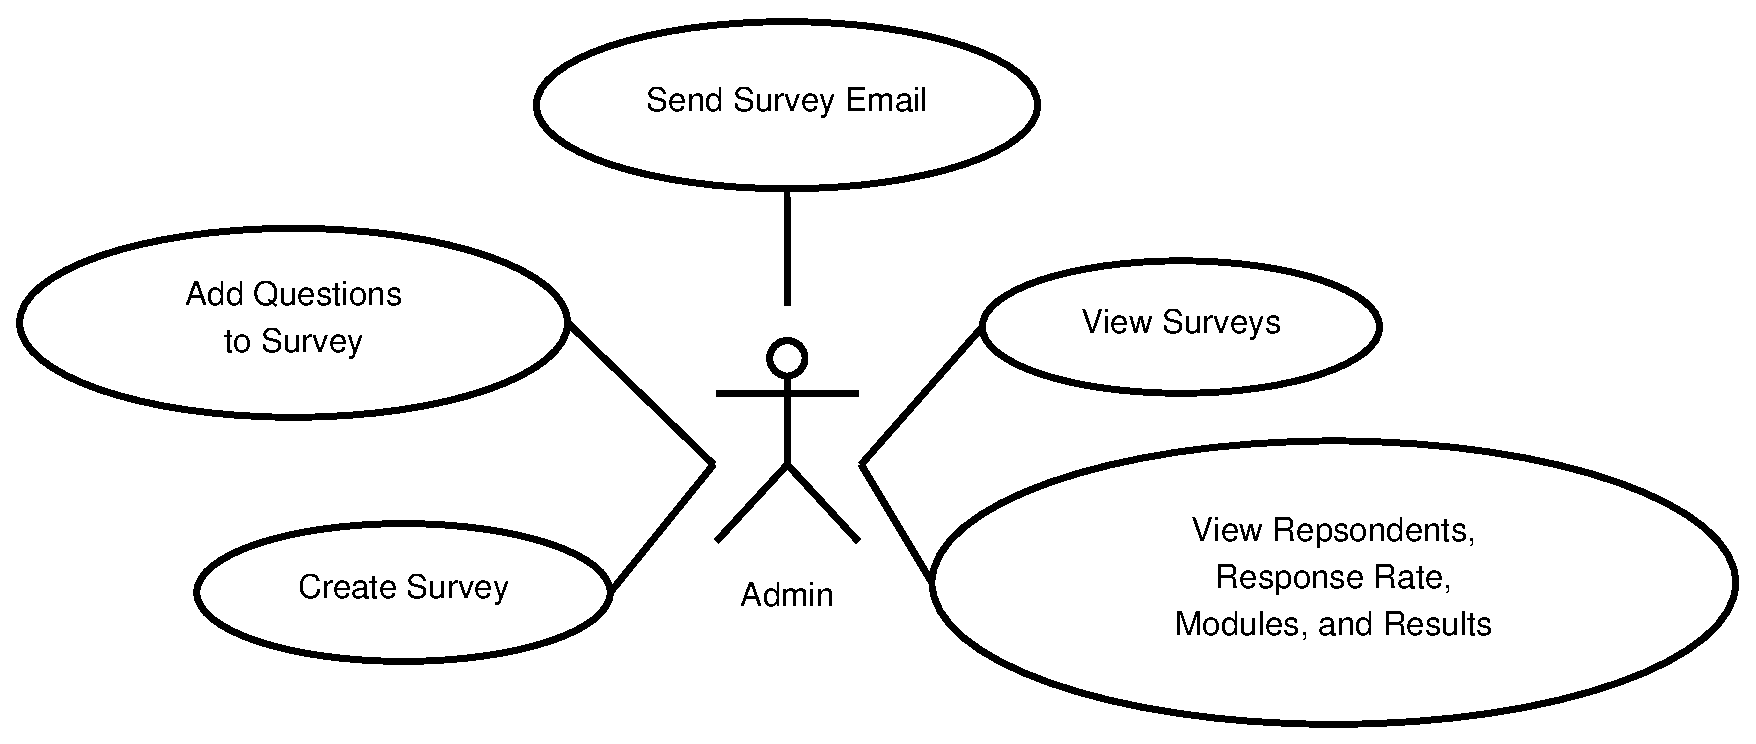
\includegraphics[width=\textwidth]{use_case-admin}
		\caption{Admin use-case diagram.}
		\label{fig:use_case-admin}
	\end{figure}
	
	\autoref{fig:use_case-admin} shows that admins can view surveys, create surveys, add questions to surveys, view more detail about survey such as respondents, response rate, modules, and results.
	They can also send an email to respondents to remind them to fill in the questionnaire.
	
	\newpage
	
	\subsubsection{Respondent User Role}
	
	\begin{figure}[H]
		\label{fig:use_case-student}
		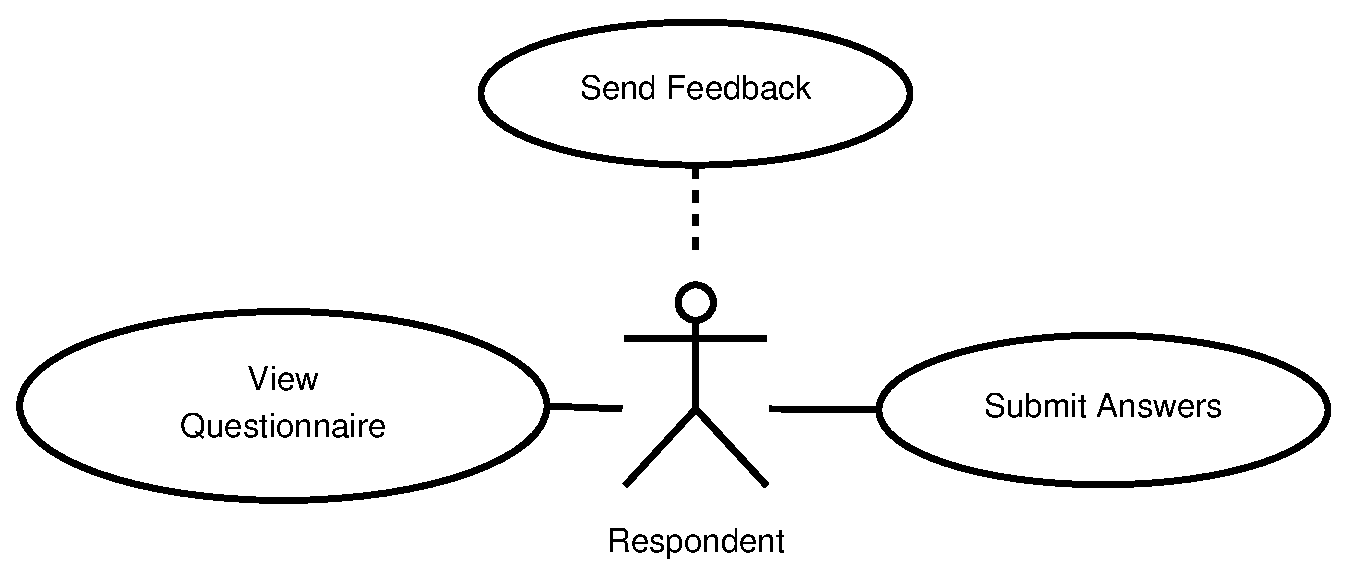
\includegraphics[width=\textwidth]{use_case-respondent}
		\caption{Respondent use-case diagram.}
	\end{figure}
	
	\autoref{fig:use_case-student} shows that a respondent only has one responsibility in the system, and that is to respond to a survey through a link sent via email.
	They can only respond once, and submitted answers cannot be seen as it would break the irreversible anonymity of the system.